% beamer presentation
% Karting report

\documentclass{beamer}
% english language
\usepackage[english]{babel}

% tables
\usepackage{tabularx}
\usepackage{graphicx}
\usepackage{hyperref}
\usepackage{listings}
\usepackage{color}

\usetheme{Madrid}

% unibs color #3d5895
% \definecolor{unibs}{RGB}{61,88,149}
\definecolor{unibs}{HTML}{3d5895}


\setbeamercolor{palette primary}{fg=white, bg=unibs}
\setbeamercolor{palette secondary}{fg=white, bg=unibs}
\setbeamercolor{palette tertiary}{fg=white, bg=unibs}
\setbeamercolor{palette quaternary}{fg=white, bg=unibs}

\title{Karting report}
\author{Denis Festa}
\date{\today}

\begin{document}


\begin{frame}
    \titlepage
    \centering
    \includegraphics[width=0.2\linewidth]{unibs-circ-logo.pdf}
\end{frame}

\logo{
\includegraphics[width=0.1\linewidth]{unibs_logo.pdf}}


\section*{User groups}

\begin{frame}
\frametitle{User groups}
\begin{figure}
    \centering
    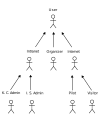
\includegraphics[width=0.4\linewidth]{drawings/users.pdf}
    \caption{User groups}
\end{figure}
\end{frame}

\section*{Use cases}

\subsection*{User}

\begin{frame}
    \frametitle{User}
    \centering
    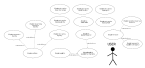
\includegraphics[width=0.9\linewidth]{drawings/uc-user.pdf}
\end{frame}

\subsection*{Intranet}

\begin{frame}
    \frametitle{Kart center administrator}
    \centering
    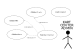
\includegraphics[width=0.9\linewidth]{drawings/uc-kcadmin.pdf}
\end{frame}

\begin{frame}
    \frametitle{Clerk}
    \centering
    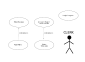
\includegraphics[width=0.9\linewidth]{drawings/uc-clerk.pdf}
\end{frame}

\begin{frame}
    \frametitle{Information system administrator}
    \centering
    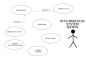
\includegraphics[width=0.9\linewidth]{drawings/uc-isadmin.pdf}
\end{frame}

\subsection*{Extranet}

\begin{frame}
    \frametitle{Organizer}
    \centering
    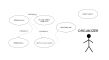
\includegraphics[width=0.9\linewidth]{drawings/uc-organizer.pdf}
\end{frame}

\subsection*{Internet}

\begin{frame}
    \frametitle{Pilot}
    \centering
    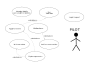
\includegraphics[width=0.9\linewidth]{drawings/uc-pilot.pdf}
\end{frame}

\begin{frame}
    \frametitle{Visitor}
    \centering
    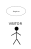
\includegraphics[width=0.3\linewidth]{drawings/uc-visitor.pdf}
\end{frame}

\begin{frame}
\frametitle{Karting center administrator}

\begin{table}
    \tiny
    \begin{tabular}{|p{2cm}|p{6cm}|}
    \hline
    Group name & \textbf{Karting center administrator} \\
    \hline
    Profile data & Name, Surname, e-mail address, password, address, phone number \\
    \hline
    Super group & Intranet \\
    \hline
    Sub group & None \\
    \hline
    Relevant use cases & CRUD on events, races, pilots, tracks, leaderboard, 
    login, logout \\
    \hline
    Read & All \\
    \hline
    Write & All \\
    \hline
    \end{tabular}
    \end{table}

\end{frame}

\begin{frame}
\frametitle{Pilot}

\begin{table}
    \tiny
    \begin{tabular}{|p{2cm}|p{6cm}|}
    \hline
    Group name & \textbf{Pilot} \\
    \hline
    Profile data & Name, Surname, e-mail address, password, address, phone number \\
    \hline
    Super group & Internet \\
    \hline
    Sub group & None \\
    \hline
    Relevant use cases & Create a race, Apply for an event, 
    login, logout \\
    \hline
    Read & All \\
    \hline
    Write & Race, Leaderboard \\
    \hline
    \end{tabular}
    \end{table}

\end{frame}


\section*{Data dictionary}
\begin{frame}
\frametitle{Data dictionary}

% Table with two columns and 9 rows:
% - Name
% - Synonym
% - Description
% - Example of instance
% - Properties
% - Components
% - Relations
% - Superconcepts
% - Subconcepts

% table 9x2
\begin{table}
\tiny
\begin{tabular}{|p{2cm}|p{6cm}|}
\hline
Name & \textbf{Karting center} \\
\hline
Synonym & Go-karting center \\
\hline
Description & Karting center \\
\hline
Example of instance & 
Name: Mantova Karting Center \newline
\textit{City}: Mantova \newline
\textit{nPilots}: 5937 \newline
\textit{nRaces}: 12485 \newline
\textit{nEvents}:74 \newline
\textit{avgReviewScore}: 3.9 \\
\hline
Properties & 
Name: the name of the karting center\newline
\textit{City}: the city where the karting center is located\newline
\textit{nPilots}: the number of pilots that have raced in the karting center \newline
\textit{nRaces}: the number of races that took place in the karting center \newline
\textit{nEvents}: the number of events that had at least one race hosted by the karting center \newline
\textit{avgReviewScore}: the average score of the reviews of the karting center \\
\hline
Components & None \\
\hline
Relations &
KartingCenter\_City (N:1): the city where the karting center is located \newline
KartingCenter\_KartingCenterAdmin (N:1): the karting center administrator of the karting center \newline
KartingCenter\_Clerk (1:N): the clerks of the karting center \newline
KartingCenter\_KartingCenterReview (1:N): the reviews of the karting center \newline
KartingCenter\_Track (1:N): the tracks of the karting center \\
\hline
Superconcepts & None \\
\hline
Subconcepts & None \\
\hline
\end{tabular}
\end{table}

\end{frame}

\begin{frame}
\begin{table}
\tiny
\begin{tabular}{|p{2cm}|p{6cm}|}
\hline
Name & \textbf{City} \\
\hline
Synonym & None \\
\hline
Description & City \\
\hline
Example of instance & 
Name: Mantova \\
\hline
Properties & 
Name: the name of the city \\
\hline
Components & None \\
\hline
Relations &
City\_KartingCenter (1:N): the karting centers located in the city \newline
\textit{City\_Track} (1:N): the tracks (inside a karting center) located in the city \newline
\textit{City\_Event} (N:N): the events that had at least one race on a track of a karting center
located in the city \\
\hline
Superconcepts & None \\
\hline
Subconcepts & None \\
\hline
\end{tabular}
\end{table}
\end{frame}

\begin{frame}
\begin{table}
\tiny
\begin{tabular}{|p{2cm}|p{6cm}|}
\hline
Name & \textbf{Track} \\
\hline
Synonym & Circuit \\
\hline
Description & Track \\
\hline
Example of instance &
Name: T1 \newline
Length: 700m \newline
\textit{City}: Mantova \newline
\textit{AsphaltType}: resin \newline
\textit{nRentalGoKarts}: 23 \newline
\textit{Difficulty}: Intermediate \newline
\textit{nPilots}: 3873 \newline
\textit{nRaces}: 7437 \newline
\textit{nEvents}: 43 \newline
\textit{avgReviewScore}: 4.2 \\
\hline
Properties &
Name: the name of the track \newline
Length: the length of the track \newline
\textit{City}: the city where the karting center the track belongs to is located \newline
\textit{AsphaltType}: the type of asphalt of the track \newline
\textit{nRentalGoKarts}: the number of rental go-karts available in the track \newline
\textit{Difficulty}: the difficulty of the track \newline
\textit{nPilots}: the number of pilots that have raced on the track \newline
\textit{nRaces}: the number of races that took place on the track \newline
\textit{nEvents}: the number of events that had at least one race on the track \newline
\textit{avgReviewScore}: the average score of the reviews of the track \\
\hline
Components & 
Timetable: the timetable of the track \newline
Leaderboard: the leaderboard of the track \\
\hline
Relations &
Track\_KartingCenter (N:1): the karting center the track belongs to \\
\hline
Superconcepts & None \\
\hline
Subconcepts & None \\
\hline
\end{tabular}
\end{table}
\end{frame}




% Quando voglio visitare un nuovo arrivo
% utilizzo non una query ma una derivata
% che calcola la query una volta sola

\end{document}